\chapter{Cartes de réionisation}

Nous avons abordé dans la partie précédente une étude centrée sur les halos.
Cependant les contraintes observationnelles sur la réionisation ne sont pas basées sur les halos mais sur l'\ac{IGM}, (voir \ref{sec_contraintes_obs}) et donc sur les régions sous-dense loin des halos.
Nous nous intéressons dans cette section à un aspect complémentaire de ceux abordés dans les parties précédentes, l'histoire de l'état d'ionisation de l'\ac{IGM}.
Cette histoire est contenue dans un outils essentiel de l'étude de la réionisation dans son ensemble, les cartes de redshift d'ionisation.
Ces cartes sont constituées en chaque point de l'espace, du redshift auquel chaque cellule est passée au dessus d'un certain niveau d'ionisation moyen.
%Les cartes de redshift de réionisation sont de outils important pour l'étude de la réionisation dans son ensemble.

Nous allons voir dans ce chapitre comment j'ai implémenté le calcul des cartes de réionisation dans EMMA.
Je présenterai ensuite une méthode pour déterminer la vitesse des front d’ionisation.


\section{Méthode de calcul des cartes}

Les cartes de redshift contiennent pour chaque cellules le redshift auquel elles a été ionisée.
Il est possible de calculer ces cartes à partir des sorties mais dans le but d'obtenir la meilleur résolution temporelle possible, j'ai implémenté dans EMMA le calcul des cartes de réionisation à la volée, pendant l'exécution d'une simulation.
L'instant à conserver sera définis par le passage de la fraction d'ionisation de la cellule par un seuil.
Ce seuil sera définis à  50\% par la suite.
Comme certaines cellules peuvent recombiner, il existe deux façons de définir un redshift de reionisation: il est possible de considérer soit la première, soit la dernière ionisation:
L'implémentation est présenté sur le Listing \ref{lst:majz}.

\begin{itemize}
\item Dans le cas de la première ionisation, la valeur ne devra être mise a jour qu'une seule fois au moment du passage du seuil.
Pour ce faire, toutes les cellules seront initialisées à une valeur caractéristique (eg -1).
La mise à jour ne se fera donc qu'à la condition que la fraction d'ionisation soit supérieure au seuil et que la valeur actuelle du redshift d'ionisation soit -1.
Ainsi la valeur ne sera pas remise à jour à chaque pas de temps où la cellule sera ionisée. 

\item Dans le cas de la dernière ionisation, la valeur du redshift sera mise à jour, tant que la fraction d'ionisation de la cellule est inférieure au seuil.
Ainsi, si un cellule recombine, le valeur de son redshift associé sera de nouveau mise à jour, et la mise à jour stoppera à chaque passage au dessus du seuil.
\end{itemize}

\begin{lstlisting}[float=bth,language=c,frame=tb,caption={Mise a jour du redshift de reionisation},label=lst:majz]
  #define THRESH_MAP (0.5)

  if(cell.xion<THRESH_MAP)
    cell.t_last_xion=current_t;

  if( (xion>=THRESH_MAP) && (cell.t_first_xion==-1) )
    cell.t_first_xion=current_t;
\end{lstlisting}


Dans le cas d'une grille \ac{AMR}, l'organisation de la grille est amenée à évoluer.
La question du raffinement/deraffinement se pose alors.
Si dans le cas du raffinement, l'injection directe du redshift de la cellule mère ne pose pas de problème particulier, les choses sont différentes lors du déraffinement.
En effet, dans EMMA, quand une cellule est deraffinée la valeur moyenne des 8 cellules filles est injectée dans la cellule mère (voir \ref{Opérateurs de changement de grilles}).
Le problème est que les processus physiques qui ont lieu dans la simulation sont calculés par rapport au temps et que les redshift ne sont pas linéaire en temps (voir \ref{sec:friedman}).
Ainsi les redshift ne doivent pas être moyennés.
Pour résoudre ce problème, j'ai fait le choix de travailler non pas avec le redshift mais avec l'age de l'Univers au moment de l'ionisation de la cellule.
Les cartes de temps pourront être converties en cartes de redshift en post traitement en utilisant les mèmes paramètres cosmologiques que ceux utilisés en interne de la simulation.

Un exemple de carte de première réionisation obtenue est présenté sur le figure \ref{fig:zmap}.
Cette carte a été générée a partir d'une simulation présentant des caractéristiques similaires a celles des simulation présentées au chapitre précédent (voir section \ref{sec:pres_simu}).
Elle a un volume de $\left( 8h^{-1} \mathrm{cMpc} \right) ^3$ et est exécutée sans feedback de supernovae. 
On y observe des motifs concentriques et asphérique autour des sources. 
Ces motifs présentent une forme de "papillon" dû à la non homogénéité du gaz, la présence de filaments ralentissant le rayonnement autour des sources.

\begin{figure}
        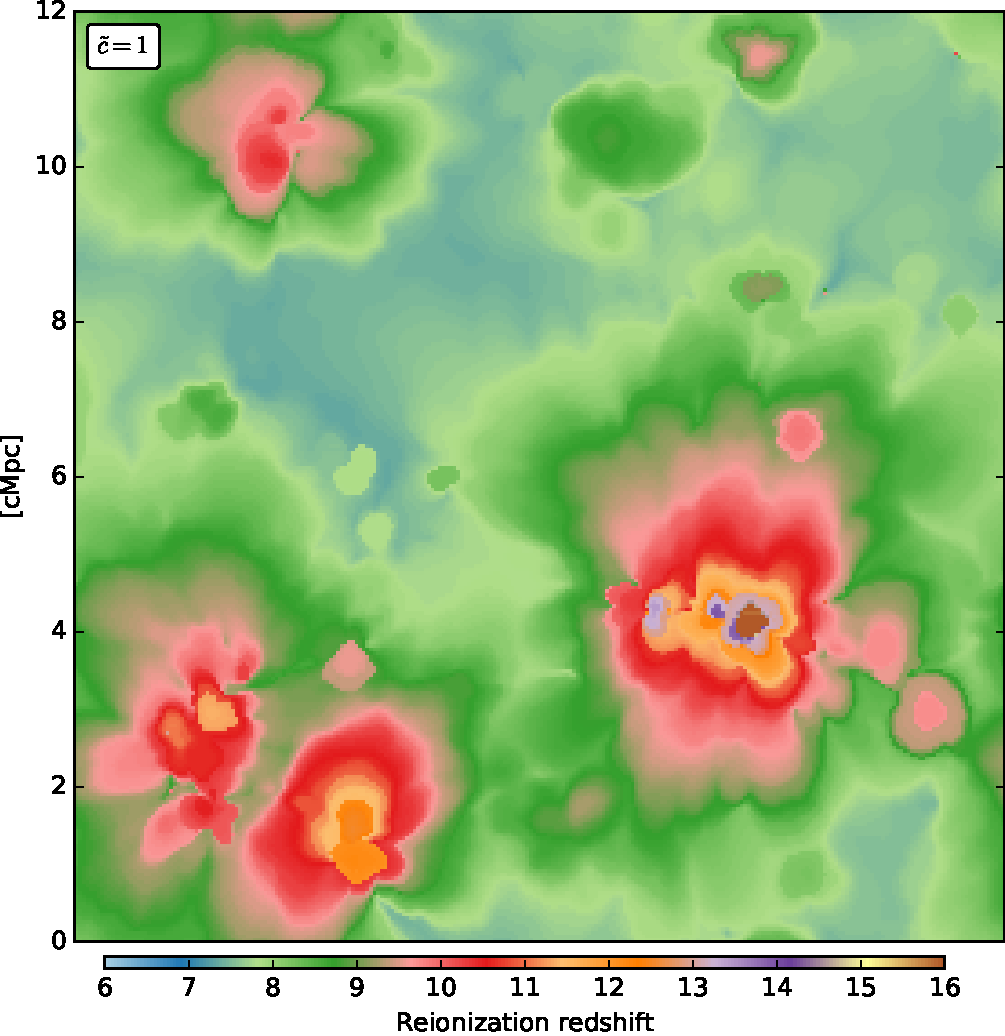
\includegraphics[width=.95\linewidth]{img/04_mapreio/map_z_c1.pdf} 
        \caption[Carte de redshift d'ionisation]{Exemple de carte de redshift d'ionisation générée par EMMA.
        Cette carte contient toute l'histoire de réionisation de la simulation.
        Il s'agit d'une tranche d'une cellule d'épaisseur centrée sur la première cellule ionisée.
 		\label{fig:zmap}}
\end{figure}

\clearpage
\section{Cartes de vitesse d’ionisation}

Partant du principe que les cartes de redshift d'ionisation contiennent l'information de toute l'évolution de la fraction d'ionisation de la simulation, il est possible de remonter à la vitesse de propagation des fronts d'ionisation.
%À partir des cartes de redshift de réionisation
%L'idée est la suivante:
En utilisant le fait que les cartes de réionisation donnent un temps pour chaque point de l'espace, il est possible de déterminer quel est le temps qu'il s'est écoulé entre la réionisation de deux cellules adjacentes, et donc de connaître la vitesse à laquelle le front d'ionisation les a traversées.
En pratique, la vitesse des fronts sera obtenue en calculant le gradient de la carte de réionisation.
Le gradient représente le temps $dt$ mis par le front pour parcourir une distance $dx$ correspondant à la taille de la cellule.
Par soucis de simplicité, et comme le calcul du gradient est problématique au niveau des interfaces entre niveaux de raffinement, les études présentées ici ont été réalisées en projetant la grille \ac{AMR} sur le niveau de base, de manière à n'avoir qu'un seul niveau, et à supprimer ces interfaces.
L'objectif est de comparer la vitesse des fronts d'ionisation à la vitesse de la lumière.
%Pour obtenir directement une vitesse il est préférable de travailler en temps et non en redshift.
%Or il reste un problème à régler, la carte de vitesse obtenue est en unité comobile, alors que la lumière voyage avec une vitesse physique.
La carte de vitesses obtenue étant en unités comobile, le gradient devra être pondéré par la valeur du facteur d'expansion au moment de l'ionisation de la cellule associée.
%On obtiendra ce facteur par intégration de la cosmologie, de la même façon que pour transformer la carte de temps en carte de redshift.

Le gradient sera discrétisé de la manière suivante:

\begin{equation}
\vec{\nabla} t_{reio}^i \approx \frac{t^{i+1}  - t^{i-1}}{2a^i \left( x^{i+1}  - x^{i-1} \right)}.
\end{equation}

ou $i$ est l'indice de la cellule, a le facteur d'expansion, $t$ le temps d'ionisation et $x$  la position de la cellule.
La vitesse des fronts d'ionisation $V_{reio}$ est alors définie comme l'inverse de la norme de ce gradient:

\begin{equation}
V_{reio}  = \left | \frac{1}{ \vec{\nabla} t_{reio}} \right| .
\end{equation}

Un exemple de carte de vitesses de fronts obtenue est présenté sur la figure \ref{fig:vmap}.
Comme sur la figure \ref{fig:zmap}, on y observe des motifs concentriques autour des sources.
Ces motifs sont composés d'une alternance de vitesses lente et rapide représentant les génération successives d'étoiles.

\begin{figure}
        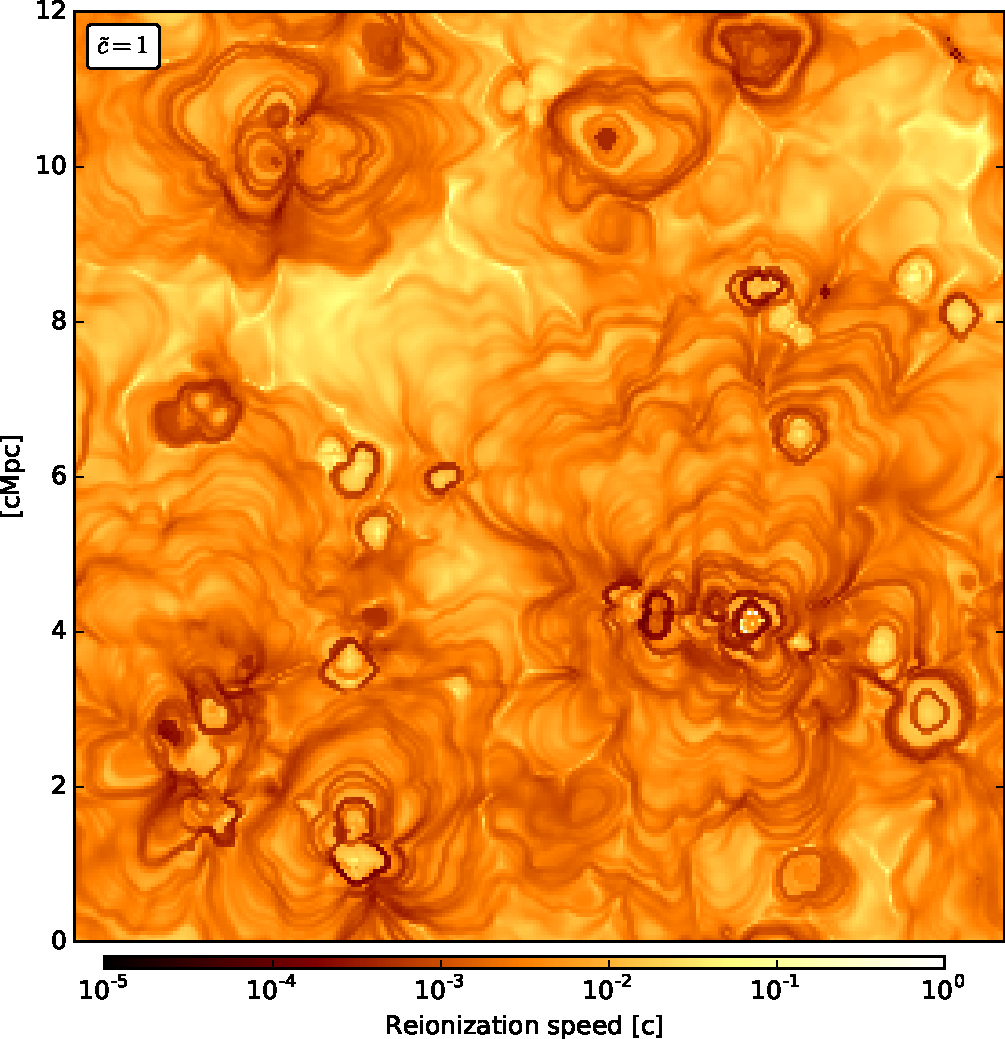
\includegraphics[width=.95\linewidth]{img/04_mapreio/map_v_c1.pdf} 
        \caption[Carte de vitesse des fronts d'ionisation]{Exemple de carte de vitesse de fronts générée par la méthode du gradient.
		 Cette carte correspond a la même tranche que celle présenté Figure \ref{fig:zmap}
        }
 		\label{fig:vmap}
\end{figure}

Cette méthode du gradient possède un biais qui peux mener à des valeurs de vitesses aberrantes dans le cas ou deux cellules adjacentes ne se font pas ioniser par la même source.
Ceci peux arriver dans deux cas : 
\begin{itemize}
\item Proche des sources, si deux particules stellaires sont formées en même temps dans deux cellules voisine.
\item Loin des sources, au moment de la rencontre entre deux fronts d'ionisation.
\end{itemize}

Dans ces deux cas il est possible d'avoir deux cellules voisine avec le même redshift d'ionisation.
Ce qui mène a un gradient nul et a une vitesse infinie.
En pratique, ces cas extrêmes n'arrivent que rarement avec une probabilité de l'ordre de $10^{-6}$.


\section{Vitesse des fronts en fonction du redshift}

Dans les deux sections précédentes, nous avons associé a chaque cellule un redshift et une vitesse.
Regardons maintenant comment se comporte l'un par rapport a l'autre sur la Figure. \ref{fig:speedz}.

On observe que la gamme de vitesse des fronts est comprise entre $10^{-4}c$ et $10^{-1}c$ sur une grande partie du processus de réionisation (avant $z=8$).
Cette phase est suivie d'un pic de vitesse correspondant a une nette accélération des fronts. 
Puis, à l'instant ou toutes les cellules sont réionisées, il n'est plus possible de calculer une vitesse.

La première phase correspond a l'ionisation des zones dense.
La seconde phase correspond a l'ionisation des vides.

\begin{figure}
        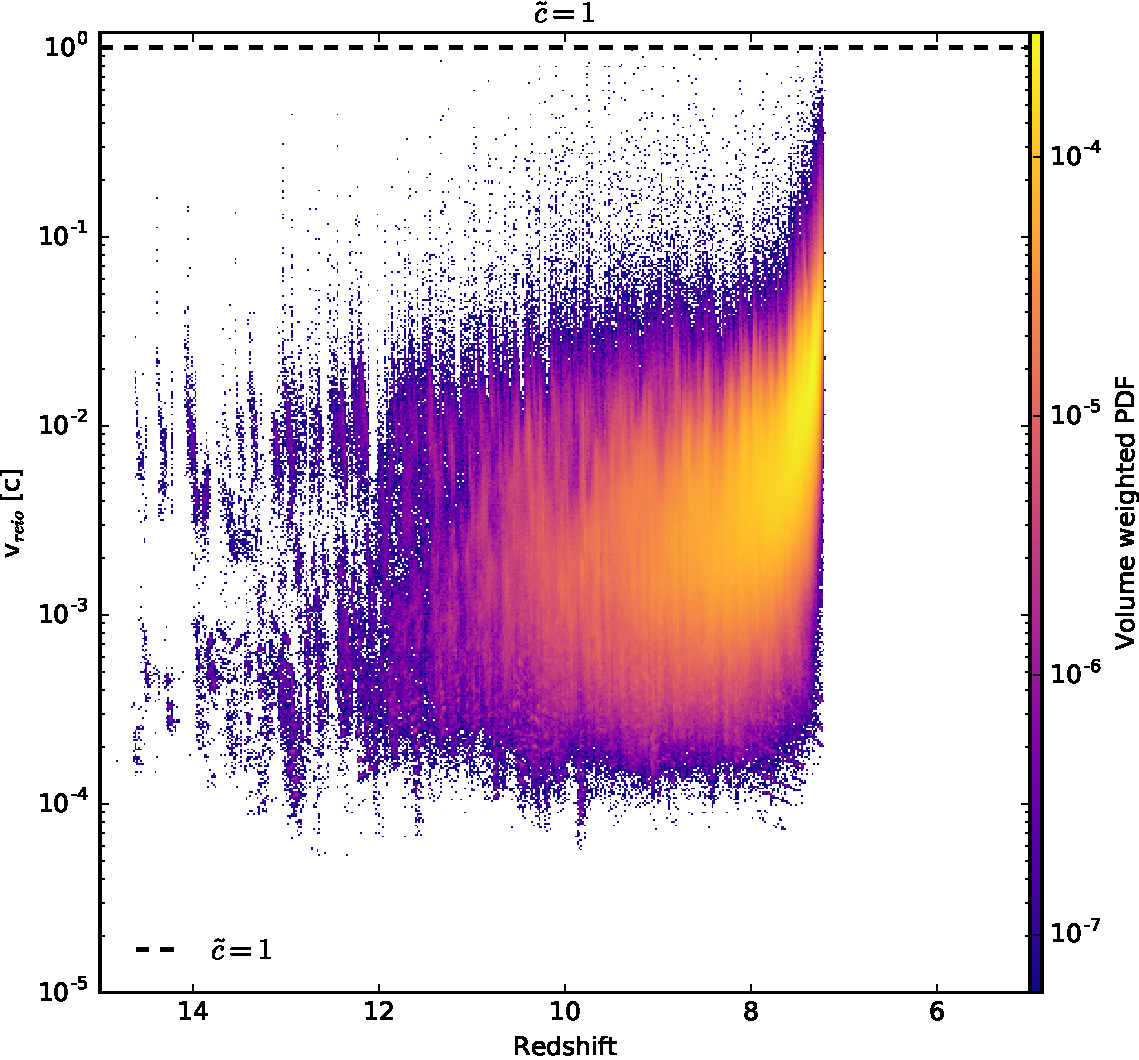
\includegraphics[width=.95\linewidth]{img/04_mapreio/speedreio_z_c1.pdf} 
        \caption[Évolution de la vitesse des fronts]{Vitesse des fronts d'ionisation en fonction du redshift.
 		\label{fig:speedz}}
\end{figure}



\section{Accélération des fronts}

Il est possible de dériver une seconde fois la carte de temps d'ionisation pour obtenir une carte d'accélération des fronts.
Comme cette seconde dérivation étant une dérivation spatiale, l'accélération obtenue est donc une variation spatiale de vitesse (en [m/s/m]).
Une carte obtenue est présentée sur la figure \ref{fig:accz}.

\begin{figure}
        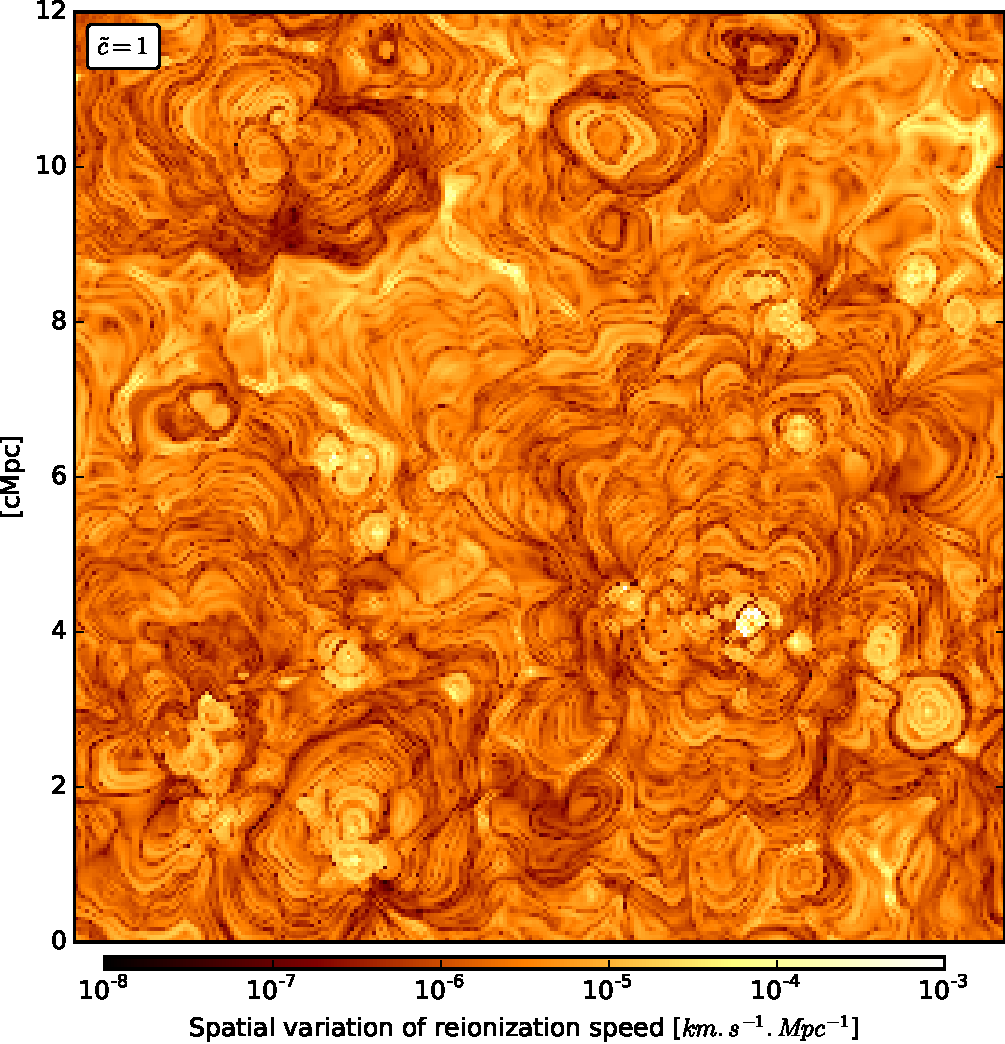
\includegraphics[width=.95\linewidth]{img/04_mapreio/map_acc_c1.pdf} 
        \caption[Accélération des fronts d'ionisation]{Carte d'accélération des fronts d'ionisation.
        Les motifs concentriques sont encore accentués.
        }
 		\label{fig:accz}
\end{figure}

Puisque la norme du gradient est représenté, cette carte n'a plus l'information de la direction de l'accélération.
On observe cependant une alternance de phases de forte accélération et de faible accélération.
Lorsque la source centrale d'un halo s’éteint, le front d'ionisation ne peu plus progresser.
Il subit donc une forte décélération.
Les valeurs d'accélérations ont tendance a être plus élevée dans les régions sous denses.

%Ces phases sont liée au temps de vie des sources

%TODO decrire la carte

De la même manière que précédemment, il est possible de lier les cartes de vitesses et d'accélération : figure \ref{fig:accspeed}.

\begin{figure}
        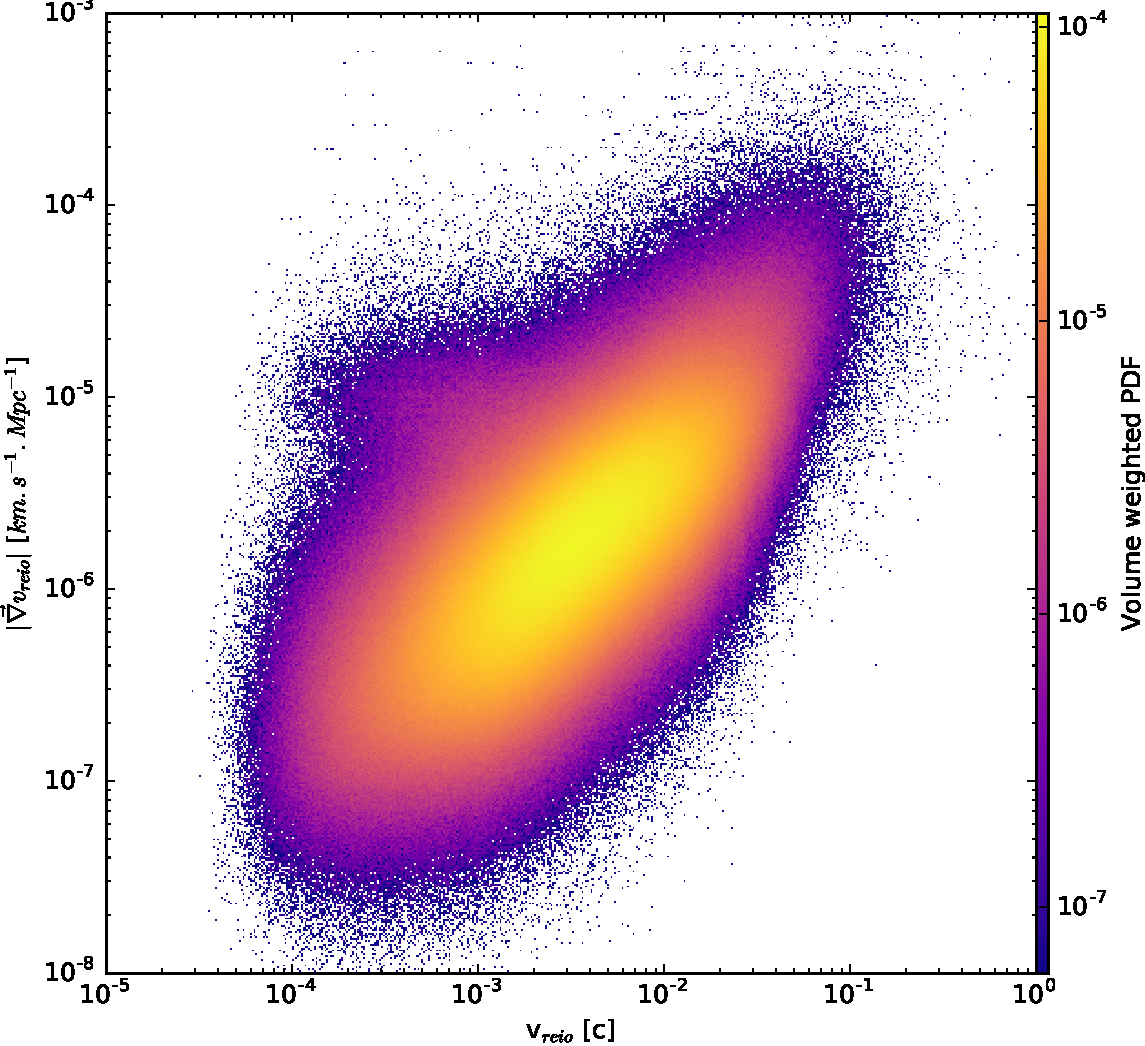
\includegraphics[width=.95\linewidth]{img/04_mapreio/v_gradv_c1.pdf} 
        \caption[Évolution de l'accélération des fronts]{Accélération des fronts d'ionisation en fonction de leur vitesse.
        Il existe une corrélation: plus un front va vite, plus il accélère.
 		\label{fig:accspeed}}
\end{figure}


Je n'ai pas réussi a identifier l'origine de la bosse
On y observe que plus un front est rapide, plus il accélère.
Ce qui conforte l'idée que la réionisation est un processus qui s'emballe.


\section{Conclusion}
Dans ce chapitre j'ai présenté la méthode de calcul des cartes d'ionisation que j'ai implémenté dans EMMA.
Ainsi qu'une méthode de détermination de la vitesses des fronts d'ionisation a posteriori.
En utilisant cette méthode, j'ai mis en évidence que la reionisation est un processus qui s’exécute en deux temps.
Premièrement une phases ou les fronts ont une vitesse constante lorsqu'il s'échappent des régions denses.
Puis une seconde phase accélérée ou la lumière atteins les régions vides.
Dans ces régions, les fronts d'ionisations peuvent atteindre une vitesse proche de celle de la lumière.

De plus j'ai montré qu'il existe une corrélation entre la vitesse d'un front et sont accélération: plus un front est rapide, plus il accélère.




%\chapter{Influence du l'approximation de vitesse de la lumière réduite sur la propagation des fronts d'ionisation}
\chapter{Vitesse de la lumière et vitesse des fronts d'ionisation.}
\label{sec:lightspeed}

Nous verrons finalement l’application de cette méthode sur la quantification de l’approximation de la vitesse de la lumière réduite (\ac{RSLA})


J'ai utilisé l'outil développé dans la section précédente pour comparer des simulation identiques a l'exception de l'approximation de la vitesse de la lumière réduite (\ac{RSLA}).

Comme abordé dans la section sur le solveur radiatif (\ref{sec:rad_solver}) le calcul de la radiation est coûteux en terme de ressource de calcul.
Ceci car la condition de Courant impose d'exécuter un grand nombre de pas de temps.
L'idée de la \ac{RSLA} est que la vitesse de la lumière est significativement plus rapide que la vitesse des autres processus a l’œuvre dans la simulation (hypothèse Newtonienne).
Partant de ce constat, même en la réduisant d'un facteur $N$, cette vitesse devrait rester significativement supérieure, et mener aux même résultats.
En divisant la vitesse par un facteur $N$, on peux augmenter la taille du pas de temps de ce même facteur, et donc diminuer le nombre de pas de temps total et le coût global du solveur radiatif.
L'objectif de cette section est d'explorer l'impact de ce facteur sur la vitesse des fronts d'ionisation.

Nous verrons que la réionisation est un processus qui s'effectue en deux phases, et que en fonction de la \ac{RSLA}, l'une ou l'autre est affectée.


Les simulations utilisées ici ont des caractéristiques identiques a celles présentées en %TODO ref
Elles ne contiennent pas de supernovae pour limiter les effets de couplage.



\begin{figure}
        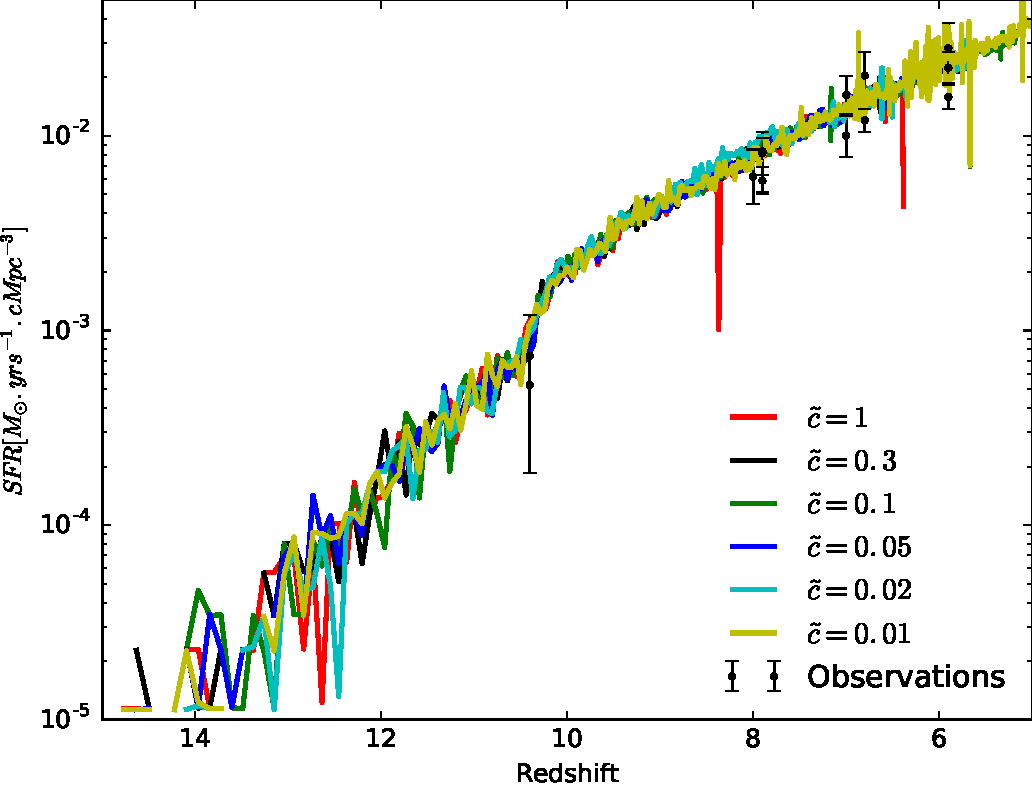
\includegraphics[height=.3\textheight]{img/04_mapreio/SFR.pdf} 
        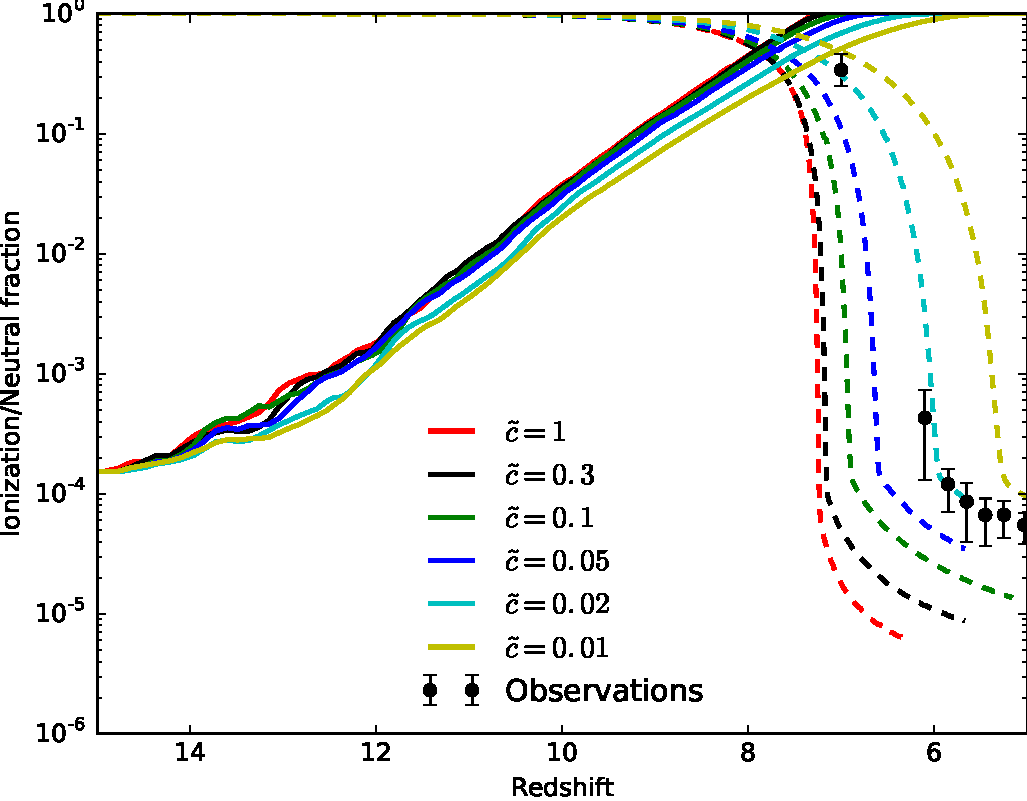
\includegraphics[height=.3\textheight]{img/04_mapreio/xion.pdf} 
        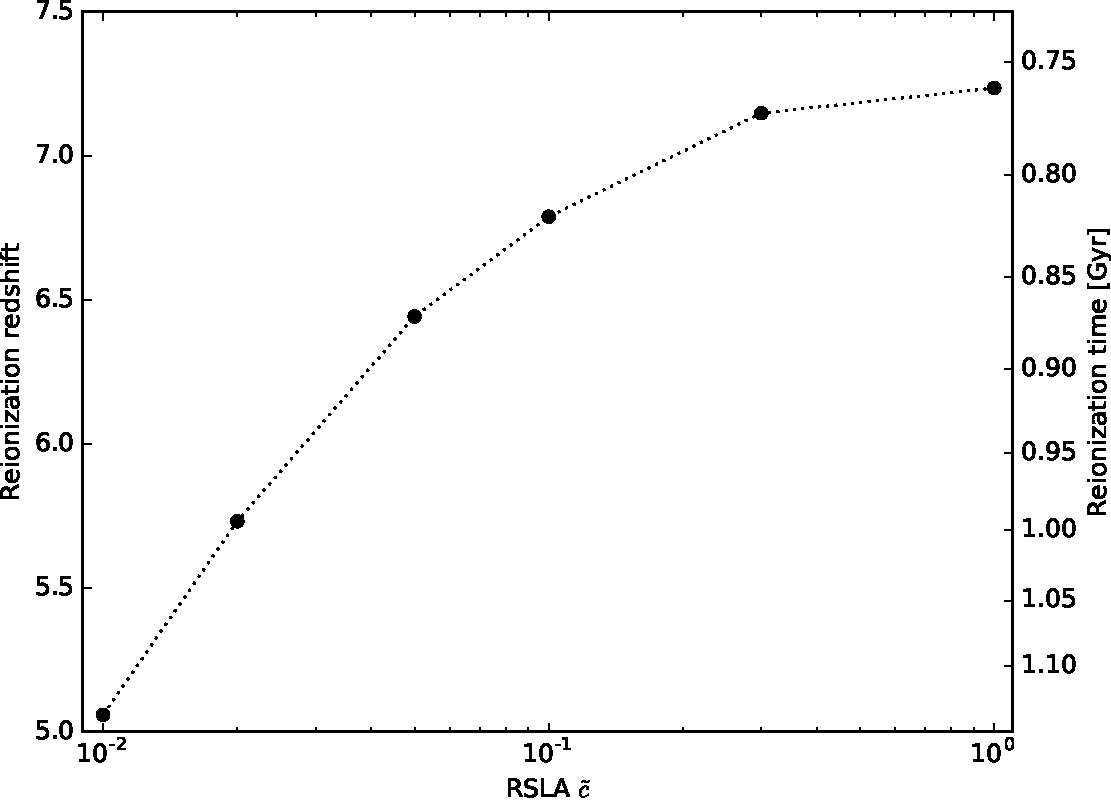
\includegraphics[height=.3\textheight]{img/04_mapreio/z_rsla.pdf} 
        \caption[Redshift de réionisation en fonction de la RSLA]{Redshift de réionisation en fonction de la RSLA
 		\label{fig:zrsla}}
\end{figure}

On observe sur le premier panneau de la figure \ref{fig:zrsla} que la \ac{RSLA} n'a pas d'impact sur la \ac{SFH} cosmique.
Dons le budget de photon n'est pas modifié entre les runs.
Cependant, on observe sur le second panneau que les histoires d'ionisation sont significativement différentes en fonction des \ac{RSLA}.
Plus la vitesse de la lumière est élevée dans la simulation, plus le volume réionise rapidement.

Cet effet a déjà été observé par \cite{rosdahl_ramsesrt_2013} par exemple qui utilise un solveur radiatif utilisant les mêmes méthodes que celui d'EMMA.

Sur le troisième volet de la figure \ref{fig:zrsla} est représenté le redshift de réionisation de la boite.
Ce redshift est définis comme étant le redshift auquel l'ionisation moyenne de la boite devient inférieur a $10^-{4}$.
On observe une certaine saturation vers les valeurs s'approchant de $\tilde{c}=1$ et une rapide croissance du redhift de réionisation quand la \ac{RSLA} diminue.


\begin{figure}
        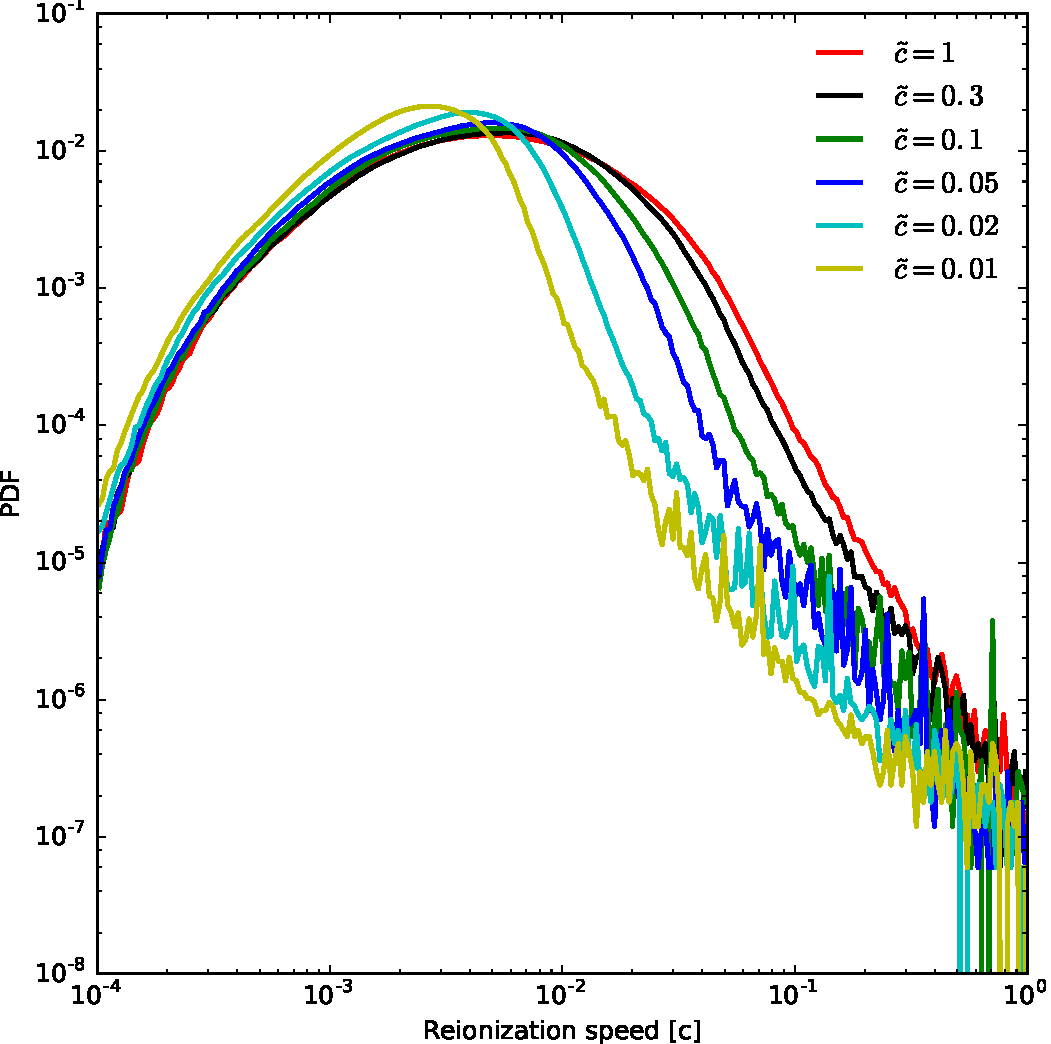
\includegraphics[width=.95\linewidth]{img/04_mapreio/PDF_v_reio.pdf} 
        \caption[PDF des vitesses de fronts]{Densité de probabilité de trouver une vitesse dans la boite.
		\label{fig:pdfv}}
\end{figure}

La figure \ref{fig:pdfv} présente la densité de probabilité de trouver une valeur de vitesse de front pour différentes \ac{RSLA}.
On y observe que diminuer la vitesse de la lumière dans la simulation n'interdit pas la présence de front plus rapide que cette vitesse mais en réduit fortement la probabilité.
Par exemple la courbe jaune corespondant à $\tilde{c}=0.01$, présente une forte décroissance 


\begin{figure}
        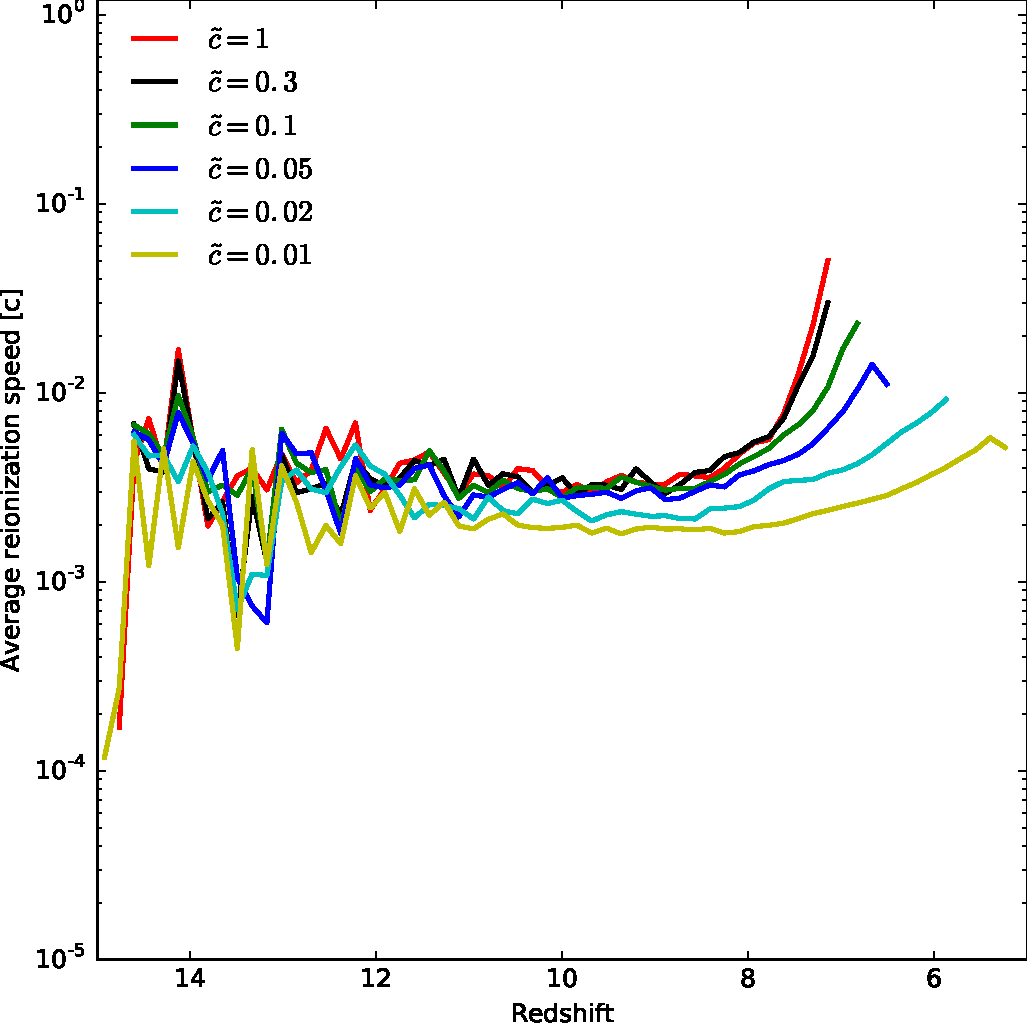
\includegraphics[width=.95\linewidth]{img/04_mapreio/avg_reionization_speed.pdf} 
        \caption[Évolution de la vitesse des fronts]{Vitesse moyenne des fronts en fonction du redshift.
        }
 		\label{fig:vreioz}
\end{figure}


\begin{figure}
        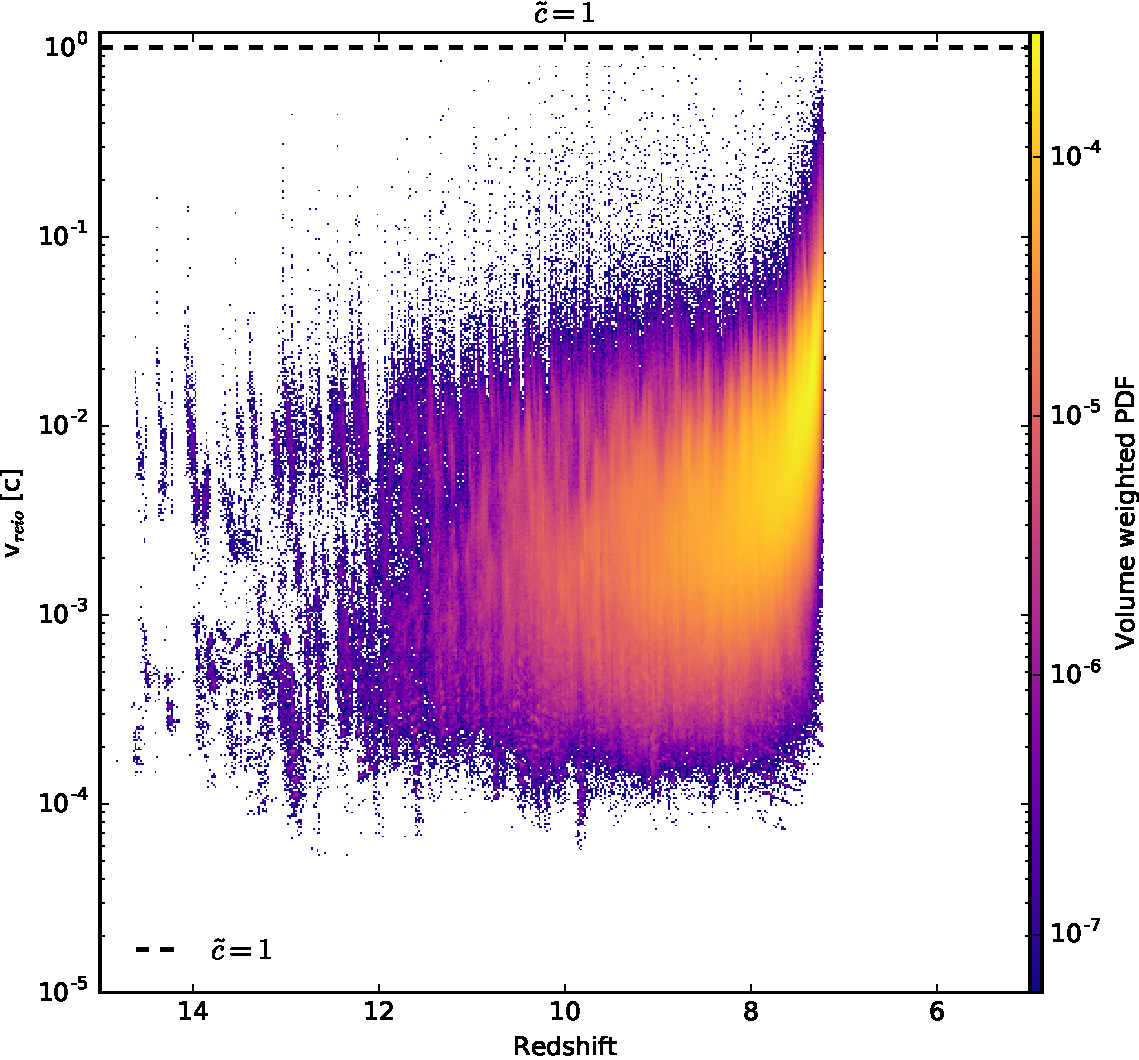
\includegraphics[height=.3\textheight]{img/04_mapreio/speedreio_z_c1.pdf} 
        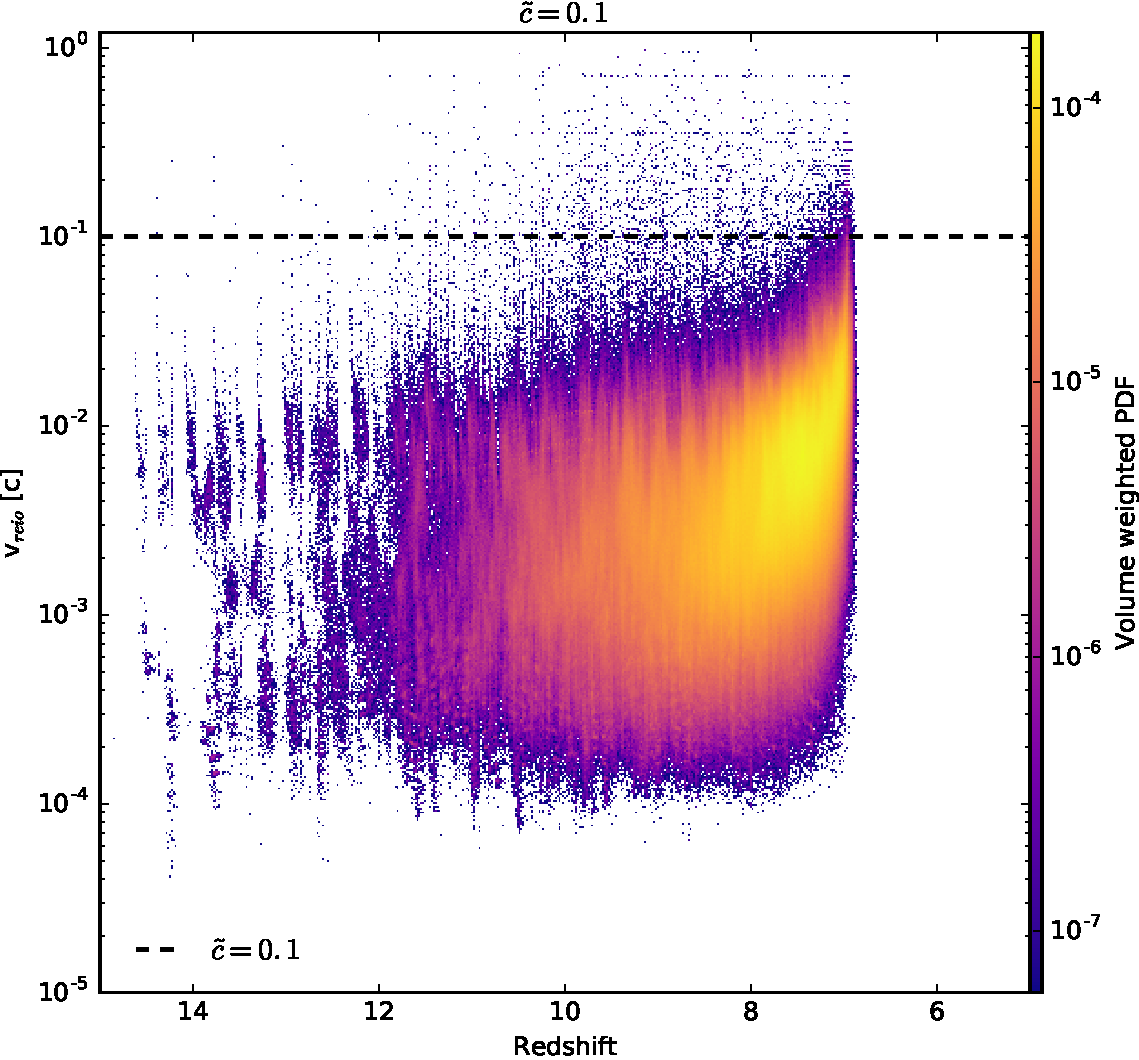
\includegraphics[height=.3\textheight]{img/04_mapreio/speedreio_z_c01.pdf} 
		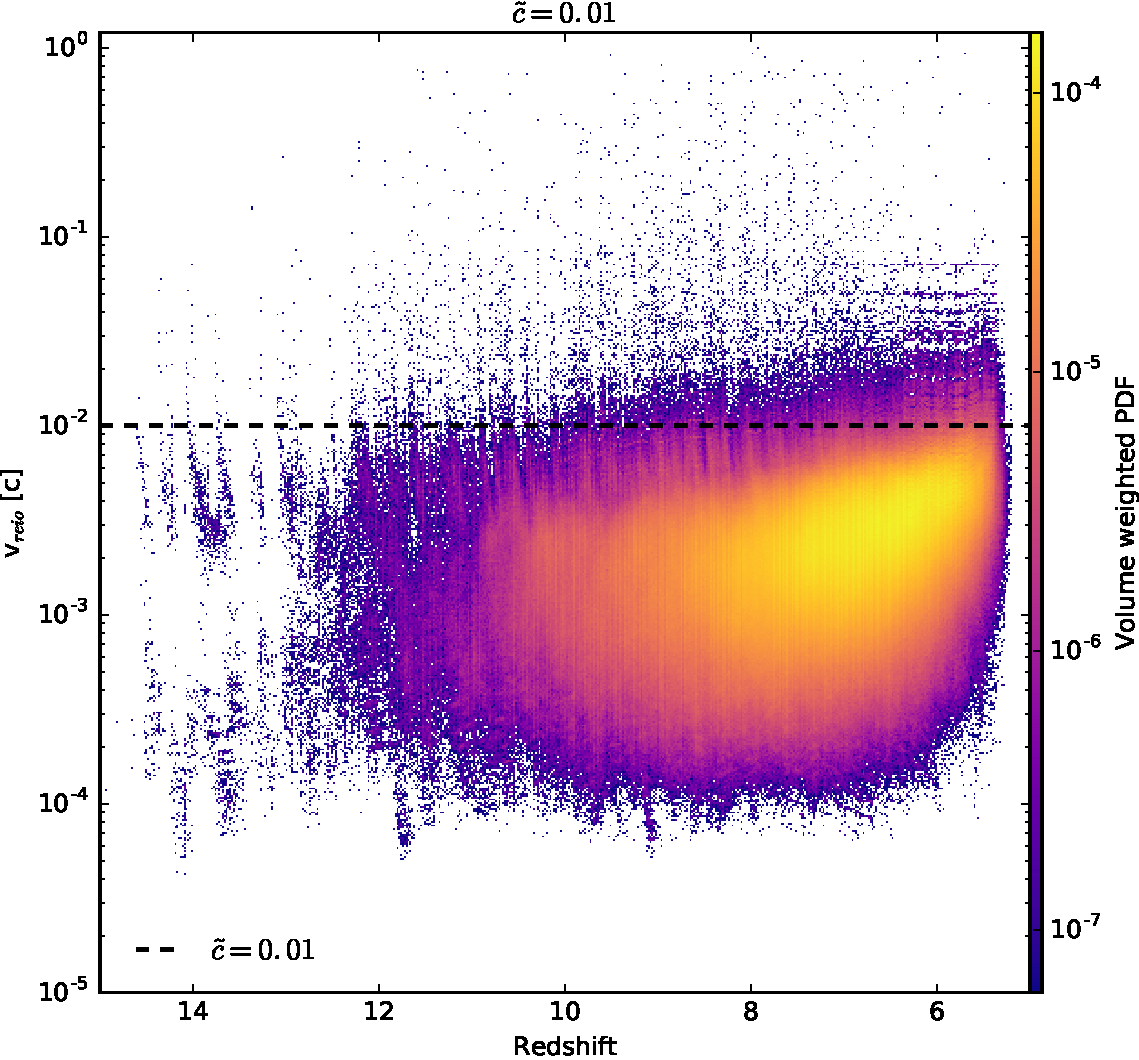
\includegraphics[height=.3\textheight]{img/04_mapreio/speedreio_z_c001.pdf} 
        \caption[Évolution de la vitesse des fronts]{Vitesse des front d'ionisation en fonction du redshift pour différentes RSLA.
        En diminuant $\tilde{c}$, on limite d'abord la seconde phase de la réionisation (l'ionisation des vide), puis la première (l'ionisation des régions denses).
        }        
 		\label{fig:vreioz}
\end{figure}



figure \ref{fig:vreioz}.

